\documentclass[12pt]{article}
\usepackage{sbc-template}
\usepackage{graphicx,url}
\usepackage[brazil]{babel}   
\usepackage[utf8]{inputenc}
\usepackage{graphicx}
\usepackage{subfigure}
\usepackage{amsmath}
\usepackage{bbm}

\title{Uma implementação do jogo Pedra, Papel e Tesoura utilizando Visão Computacional}
\author{Ezequiel França dos Santos\inst{1}, Gabriel Fontenelle\inst{1}}
\address 
{Centro Universitário Senac - Campus Santo Amaro
  (SENAC-SP)\\
  Av. Engenheiro Eusébio Stevaux, 823 -- São Paulo -- CEP 04696-000 -- SP -- Brasil
%\nextinstitute
%  Departamento de Tecnologia da Informação\\
%  Bacharelado em Ciência da Computação
  \email{{ezefranca.br,colecionador.gabriel},{(@gmail.com})}
}

\begin{document} 
\maketitle

\begin{abstract}
Space for translation, when resumo is final version % if you want translate, go ahead
\end{abstract}
     
\begin{resumo} 
Este trabalho apresenta um jogo, controlado por um algoritmo de Visão Computacional de identificação da mão (hand-tracking). O algoritmo proposto baseia-se na segmentação da imagem e construção de um fecho convexo com algoritmo de Jarvis e determinação do padrão com base em sua área e quantidade de vértices.
\end{resumo}


\section{Introdução}

A busca por meios que tornem os jogos mais interativos tem sido muito explorada na industria atual de jogos eletrônicos. Nessa área a Visão Computacional tem se destacado, permitindo a captura de gestos para uso como controle em interfaces interativas. Os dispositivos comerciais atuais de interação baseados em gestos utilizam equipamentos caros e
muitas vezes requerem ambientes especiais que dificultam a difusão destas interfaces de controle.
Este trabalho apresenta um estudo sobre a viabilidade de utilização de uma webcam como dispositivo de interação baseado em gestos da mão, especificamente para o jogo Pedra, Papel e Tesoura.


\section{Objetivos}

O objetivo é o desenvolvilmento de um jogo interativo controlado utilizando a webcam. 

\section{Desenvolvimento}


\subsection{Controle do Jogo}

Para reconhecer os gestos da mão foi necessário submeter a imagem da camera a algumas fases de pré-processamento. O diagrama 1, mostra a sequência adotada e cada etapa será brevemente descrita no decorrer deste trabalho.  

\subsubsection{Reconhecimento de padrões}
Falar brevemente, e apresentar a idéia utilizada

\begin{figure}[ht]
\centering
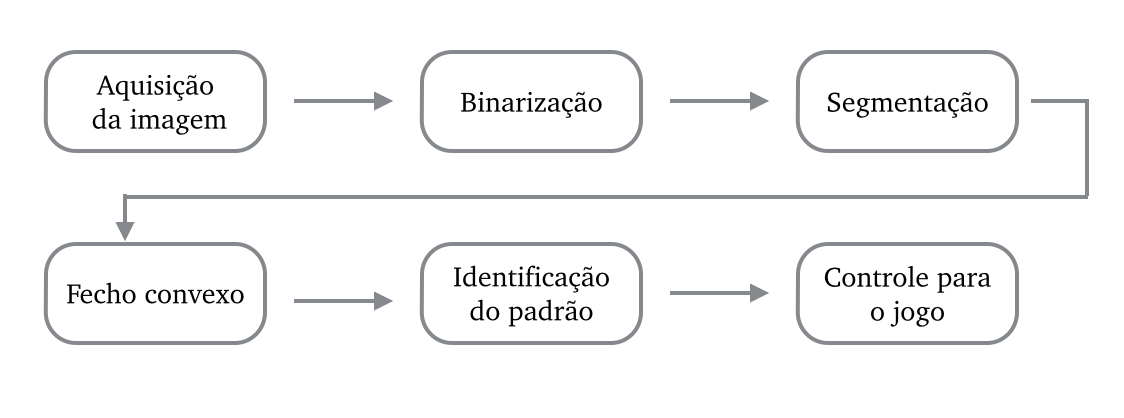
\includegraphics[width=.7\textwidth]{fluxo.png}
\caption{Fluxo no processamento da imagem} \label{fig1}
\end{figure}
\subsubsection{Aquisição da imagem}
Falar da aquisição da imagem, opencv, etc.

\subsubsection{Segmentação da imagem}

\subsubitem{Normalização para escala de cinza}
A primeira fase de pré-processamento trata-se da normalização da imagem colorida para tons de cinza. A normalização foi feita com base no valor médio dos canais de cores da imagem, conforme a equação \ref{eq:normalizacao}.



\begin{equation} \label{eq:normalizacao}
Valor{_{cinza}}{_{i, j}}= \sum_{1}^{n} \left |\frac{R + G + B}{3}\right |{_{i, j}}
\end{equation}

$Onde:\\$
$Valor{_{cinza}} -\; valor\,entre\,0\,-\,255\,para\,a\,escala\,de\,cinza$\\
$R -\; valor\,vermelho\,do\,ponto$\\
$G -\; valor\,verde\,do\,ponto$\\
$B -\; valor\,azul\,do\,ponto$\\
$n -\; quantidade\,de\,pontos\,da\,imagem$\\
$i, j \,-\;coordenadas\, (x,y)\, do\, ponto\, na\, imagem$\\

A Figura \ref{fig2} apresenta o resultado deste processo.

\begin{figure}[ht]
\centering
\mbox{\subfigure{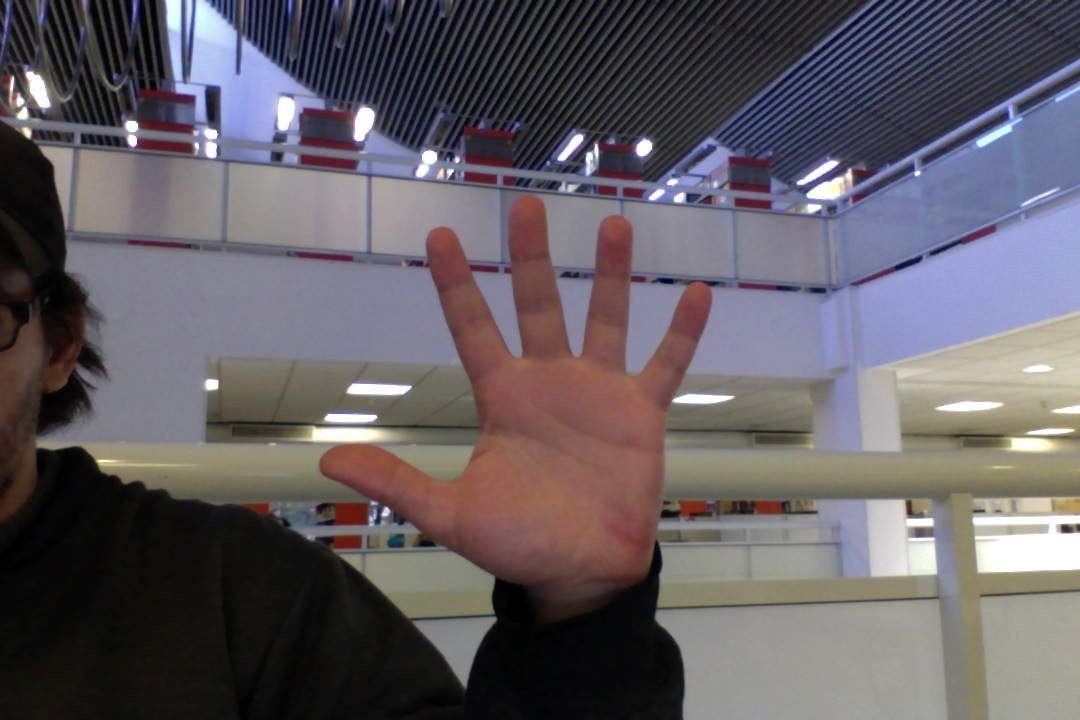
\includegraphics[width=3in]{normal.jpg}}\quad
\subfigure{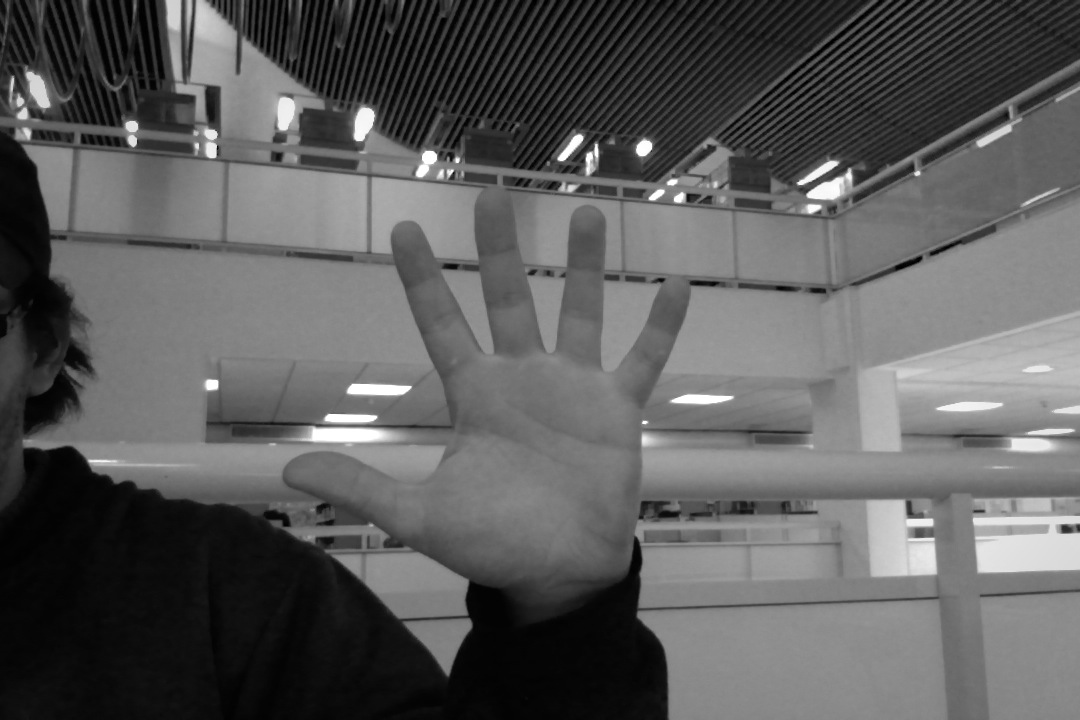
\includegraphics[width=3in]{cinza.jpg} }}
\caption{Imagem normal e imagem normalizada em cinza} \label{fig2}
\end{figure}

\subsubsection{Binarização da imagem}

Existem diversos algoritmos para binarização de imagens, dentre a lista de soluções para este  o algoritmo de Otsu, por ser de fácil implementação e apresentar resultados satisfatórios nos experimentos realizados. O algoritmo de Otsu encontra um nível de cinza $t$ tal que a soma ponderada da variância dentro das classes.
Uma desvantagem de utilizar este algoritmo é a influência da média de todo os pixeis da imagem. Isto pode fazer com que o limiar ótimo para a página toda não seja o mesmo que o de dentro de uma janela.

    \subsection{Implementação}



\subsubsection{Detecção de bordas com filtro Sobel}

O filtro Sobel calcula o gradiente da intensidade da imagem em cada ponto, dando a direcção da maior variação de claro para escuro e a quantidade de variação nessa direcção, através de duas matrizes 3x3, que são convoluídas com a imagem original para calcular aproximações das derivadas - uma para as variações horizontais $Gx$ e uma para as verticais $Gy$.
\begin{center}{Máscara de Sobel 3x3}
$$
Gx=\left[\begin{array}{rrr}
-1&0&+1\\
-2&0&+2 \\
-1&0&+1
\end{array}\right]\quad
Gy=\left[\begin{array}{ccc}
-1&-2&-1\\
0& 0& 0 \\
+1&+2&+1
\end{array}\right]
$$
\end{center}
A magnitude do gradiente é dado por:

$$
|G|=\sqrt{Gx^2 + Gy^2}
$$	


\subsubsection{Determinação do fecho convexo}
\begin{itemize}

\item Um conjunto ${\cal S} \subset {\cal R}^d$ é {\em convexo} se $\lambda
z_1 + (1-\lambda)z_2 \in {\cal S}$ sempre $z_1, z_2 \in{\cal S}$,
e $0 \le \lambda \le 1$. Resumidamente, ${\cal S}$ contém todos os segmentos de linha que conectam pares de pontos em ${\cal S}$.

\item O {\em fecho convexo} gerado por um conjunto de pontos ${\cal P}$ é
a intersecção de todos conjuntos convexos ${\cal S}$ que contem ${\cal P}$.
Se ${\cal P} = \{z_i\in{\cal R}^d, i=1\ldots, n\}$ é finito, pode ser expresso da seguinte como:

$${\cal S} = \{ \sum_{i=1}^n \lambda_i z_i \;|\; 0 \le \lambda_i \le
1, \; \sum \lambda_i = 1\}.$$

\begin{center}
\scalebox{.7}{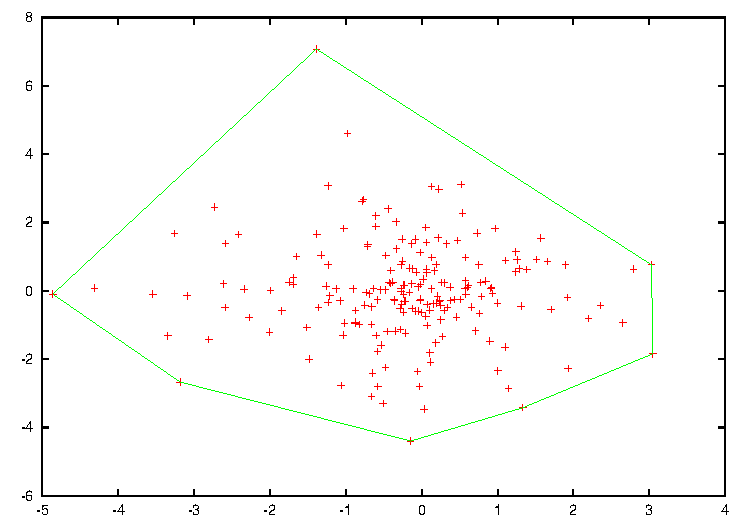
\includegraphics{fig5.pdf}}
\end{center}

\item Se ${\cal P}$ é finito, existe um único subconjunto ${\cal
P}^* \subset {\cal P}$ de tamanho mínimo de tal modo que o fecho convexo de
${\cal P}^*$ é indentico ao fecho convexo de ${\cal P}$.  O conjunto
${\cal P}^*$ é chamado de conjunto {\em gerador de fecho convexo}.

\item Encontrar o conjunto de gerador do fecho convexo de um conjunto finito ponto
${\cal P}$ é um problema computacional difícil quando a dimensão $d$
é maior que $2$.  Se a $d = 2$ existem vários algoritmos eficientes.
\end{itemize}

\bigskip
\subsubsection{Algortimo da embrulho de presente}

\begin{itemize}

\item O {\em algoritmo da marcha de Jarvis}, popularmente conhecido como {\em gift
wrapping algorithm / algoritmo do embrulho de presente} , visita os pontos do fecho convexo de maneira ordenada.

\begin{enumerate}

\item Começamos com qualquer ponto do fecho. O ponto com maior coordenada em x é uma escolha natural. Chamamos esse ponto de $(X_0, Y_0)$.

\item Varremos ("marchamos") através de todos os pontos $(X_i, Y_i)$ e localizamos o ponto tal que o ângulo a partir da coordenada $(1,0)$ para $(X_i - X_0, Y_i - Y_0)$ é minímo.
TEste é o próximo ponto de sentido anti-horário a partir de $(X_0,Y_0)$ no fecho, chamamos-o de $(X_1, Y_1)$.

\item Suponhamos que tenhamos localizado o ponto $(X_i,Y_i)$, $i=1, \ldots, m$ que ocorrem no sentido anti-horário ao fecho onde $m \ge 2$.
Calculamos todos os ângulos entre os vetores $(X_i - X_m, Y_i - Y_m)$ e
$(X_{m-1} - X_m, Y_{m-1} - Y_m)$, e procuramos o ponto $i$ que tenha o menor âgulo positivo.  Adicionamos este ponto ao fecho.

\item Retornarmos a etapa 3 até que $(X_m,Y_m) = (X_0,Y_0)$.

\end{enumerate}

\begin{center}
\scalebox{.7}{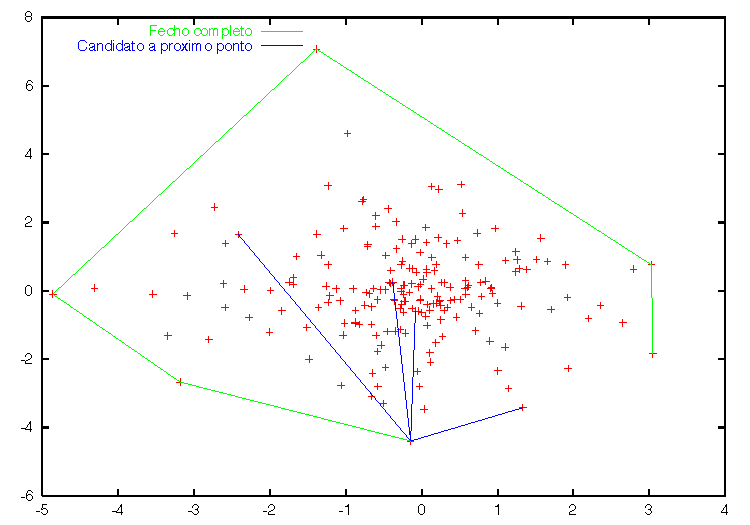
\includegraphics{figura7.pdf}}
\end{center}

\item O algoritmo de marcha Jarvis tem no pior caso complexidade O($n^2$), o que ocorre se todos os pontos estão no fecho. Em geral, se $h$ pontos estã no fecho, a complexidade é O($nh$).


\end{itemize}

\subsubsection{Calculo da área do fecho convexo}

Descrever o que inicialmente estava sendo feito (uma busca em largura), ele ficou lenta, e por isso procuramos outra alternativa, sendo o {\em shoelace} perfeito para este caso.


\begin{figure}[ht]
\centering
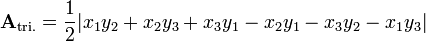
\includegraphics[width=.7\textwidth]{equacao1.png}
\label{fig:fig}
\end{figure}
\begin{figure}[ht]
\centering
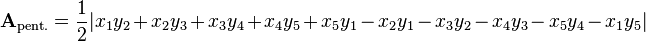
\includegraphics[width=.7\textwidth]{equcao2.png}
\label{fig:fig}
\end{figure}
\begin{figure}[ht]
\centering
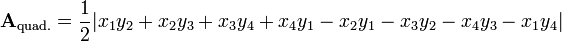
\includegraphics[width=.7\textwidth]{equacao4.png}
\label{fig:fig}
\end{figure}
\begin{figure}
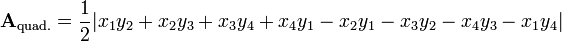
\includegraphics[width=.7\textwidth]{equacao4.png}
\label{fig:fig}
\end{figure}
\begin{figure}

\includegraphics[width=.7\textwidth]{equacao5.png}
\label{fig:fig}
\end{figure}
\begin{center}
\begin{figure}
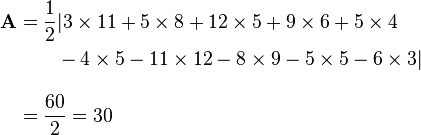
\includegraphics[width=.7\textwidth]{equacao6.png}
\label{fig:fig}
\end{figure}
\end{center}

\subsubsection{Multilinguagem}

Uso do Hash.

\subsubsection{Probabilidade Inimigo}

Minions.

\subsubsection{Pontuação}

Sobre a pontuação

\section{Resultados}

Imagens do jogo do controle (debug), imagens da pontuação e inimigos randomicos com probabilidade.

\section{Imagens do Jogo}\label{sec:figs}

\subsection{Biblioteca Allegro5}

nem sei se precisa

\subsection{Desenvolvimento de uma Engine utilizando structs}

dasdasdasdadasdas


Figure and table captions should be centered if less than one line
(Figure~\ref{fig:exampleFig1}), otherwise justified and indented by 0.8cm on
both margins, as shown in Figure~\ref{fig:exampleFig2}. The caption font must
be Helvetica, 10 point, boldface, with 6 points of space before and after each
caption.

\begin{figure}[ht]
\centering
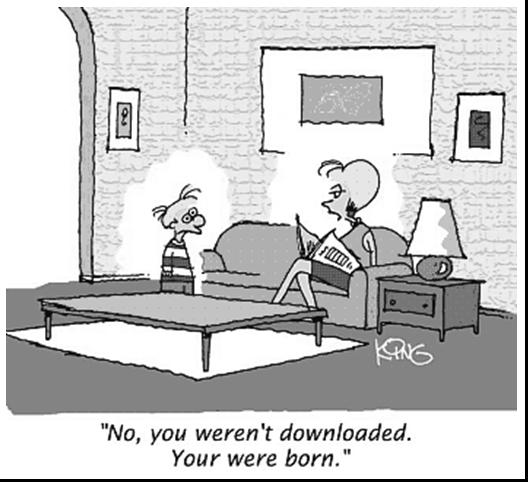
\includegraphics[width=.5\textwidth]{fig1.jpg}
\caption{A typical figure}
\label{fig:fig}
\end{figure}

\begin{figure}[ht]
\centering
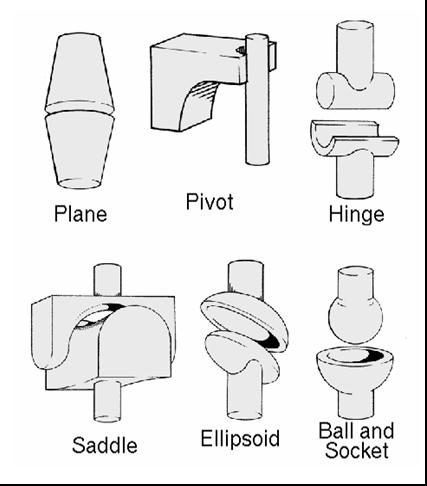
\includegraphics[width=.3\textwidth]{fig2.jpg}
\caption{This figure is an example of a figure caption taking more than one
  line and justified considering margins mentioned in Section~\ref{sec:figs}.}
\label{fig:exampleFig2}
\end{figure}

In tables, try to avoid the use of colored or shaded backgrounds, and avoid
thick, doubled, or unnecessary framing lines. When reporting empirical data,
do not use more decimal digits than warranted by their precision and
reproducibility. Table caption must be placed before the table (see Table 1)
and the font used must also be Helvetica, 10 point, boldface, with 6 points of
space before and after each caption.

\begin{table}[ht]
\centering
\caption{Variables to be considered on the evaluation of interaction
  techniques}
\label{tab:exTable1}
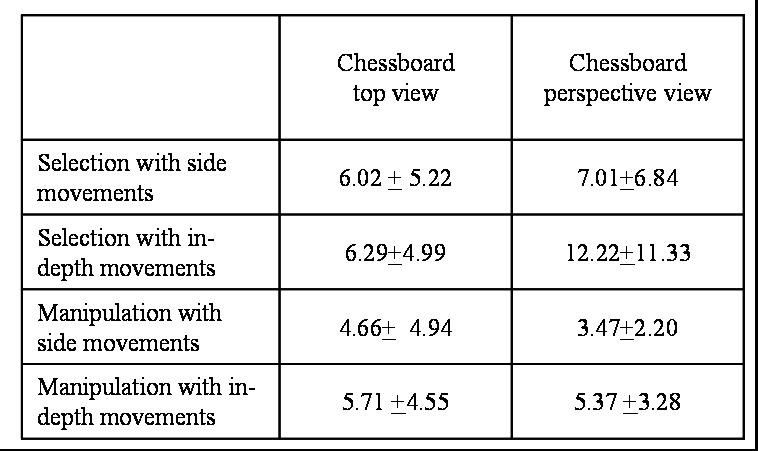
\includegraphics[width=.7\textwidth]{table.jpg}
\end{table}

\section{Conclusão}

gkgkjgkjhkjhk
hhghgjhgjhghb

\section{References}

Bibliographic references must be unambiguous and uniform.  We recommend giving
the author names references, and \cite{smith:99} \cite{barbosa:97} e \cite{rau:11}.
\cite{kishimoto:08}

SÓ LEMBRE DE ADICIONAR A BIBLIOGRAFIA CERTINHA NO ARQUIVO *.bib

\bibliographystyle{sbc}
\bibliography{sbc-template}

\end{document}
